% Synthetic fixture: a tikzpicture whose every construct is outside the
% rendered subset, under the declared refusal (`tool = none` — the
% boundary is open by default and would draw it whole otherwise). The
% engine must not let the figure collapse to whitespace: W0334 names each
% refused construct, W0362 says the whole picture is outside the subset,
% and a placeholder box marks its place — the image-placeholder precedent.
% No W0379: the declaration is the acceptance. Invented content and design.
\documentclass{article}

\pictures{ tool = none }

\fonts{ dir = "fonts", body = "Source Serif Pro" }

\begin{document}

\section{A refused diagram}

The picture below uses only constructs outside the rendered subset.

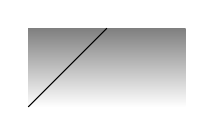
\begin{tikzpicture}
  \shade (0,0) rectangle (2,1);
  \shadedraw (0,0) -- (1,1);
\end{tikzpicture}

Text resumes after the placeholder.

\end{document}
